\section{Tasks}
\label{sec:sec006}

During our user tests, we need to ask participants to provide a subjective assessment of their experience using our \textbf{Assistant}. There are several widely used questionnaires giving us different prons-and-cons. However, in most cases, a \hyperlink{https://www.nngroup.com/articles/keep-online-surveys-short/}{single question instrument}~\cite{sauro201210} is the right method for a quantitative usability testing. By taking less time and effort to answer, participants are pursuing to this phase after task while it is minimally disruptive.

\clearpage

%%%%%%%%%%%%%%%%%%%%%%%%%%%%%%%%%%%%%%%%%%%%%%%%%%%

\hfill

\begin{wrapfigure}{r}{0.50\textwidth}
\centering
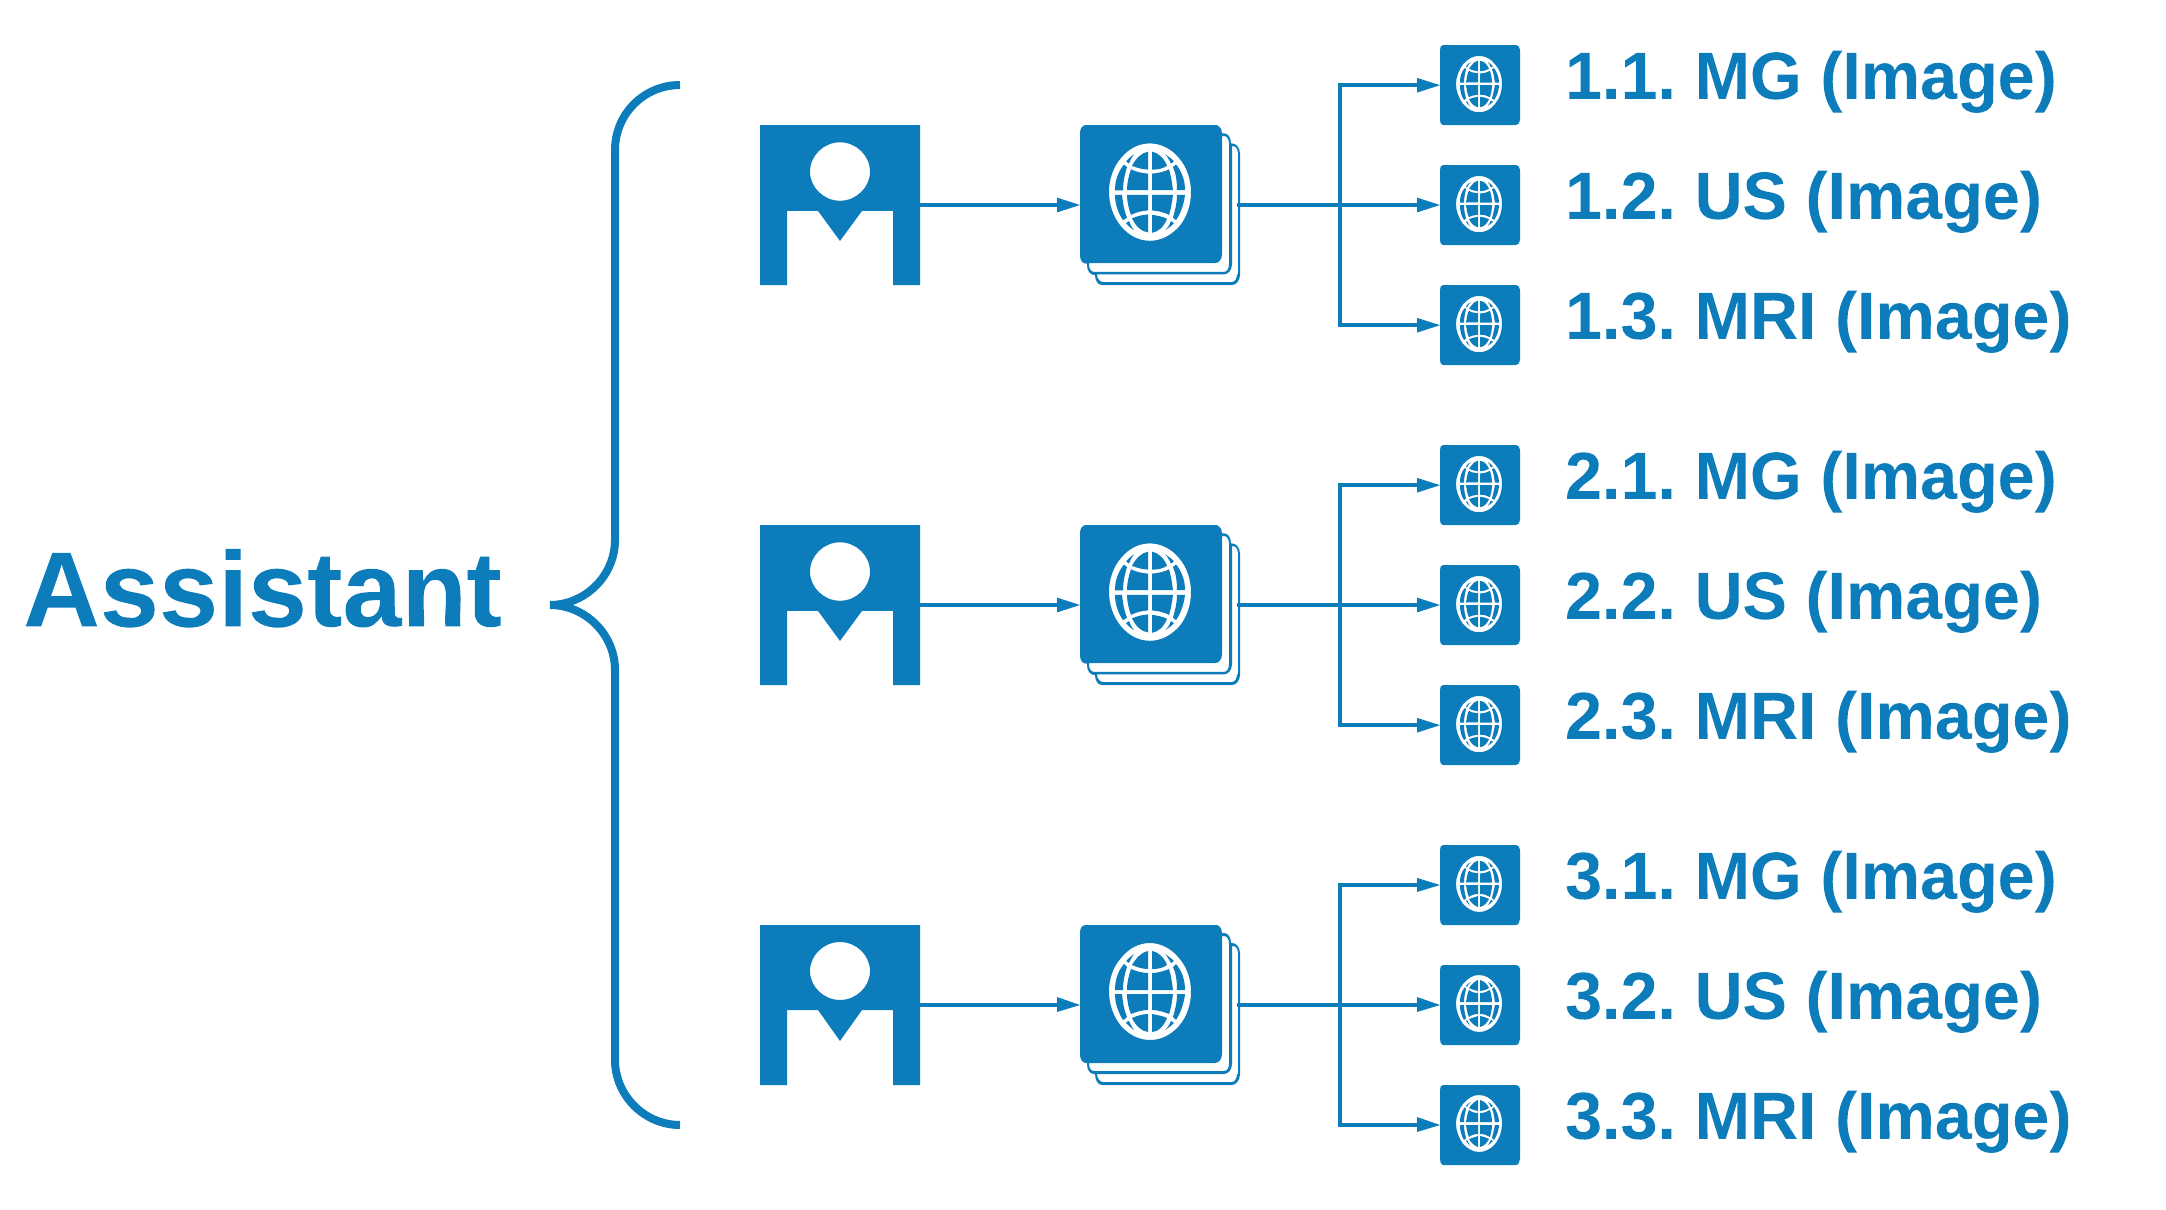
\includegraphics[width=0.50\textwidth]{img001}
\caption{Diagram representing the use of the \textbf{Assistant} by clinicians.}
\label{fig:svmm}
\end{wrapfigure}

\hfill

%%%%%%%%%%%%%%%%%%%%%%%%%%%%%%%%%%%%%%%%%%%%%%%%%%%

We will try to understand if, with the \textit{AI-Assisted} techniques, the clinicians will encounters the most accurate severity (\hyperlink{https://en.wikipedia.org/wiki/BI-RADS}{BIRADS}) of the breast lesions~\cite{american1998breast} and patient's prognostic. For this purpose, we have three patients (Figure \ref{fig:svmm}); each patient has three images in the respective modalities: (i) MG; (ii) US; and (iii) MRI. The clinicians will proceed to the activity of diagnosing the three patients within the support of our \textbf{Assistant} by the observation of ALL images.

\hfill

In our \textbf{User Testing Guide} a set of tasks is necessary and carefully crafted. Our test studies involve asking participants to perform a set of tasks. By looking at what our user need to do with our system, our tasks are realistic as possible. We are not describing the exact steps participants need to take. We achieve that by avoiding the precise language used as labels in our system. The tasks are emotionally neutrals. And we did several \hyperlink{https://www.nngroup.com/articles/pilot-testing/}{pilot tests} to prevent misleading situations saving us from wasting resources by accidentally use a lousy task or from getting bad data. The tasks are as follows.

\hfill

%%%%%%%%%%%%%%%%%%%%%%%%%%%%%%%%%%%%%%%%%%%%%%%%%%%

List of stand alone tasks:

%%%%%%%%%%%%%%%%%%%%%%%%%%%%%%%%%%%%%%%%%%%%%%%%%%%

\hfill

\begin{itemize}
\item[] \textbf{Task 1.1:} Classify \textit{Patient 1} on the \textbf{Assistant};
\item[] \textbf{Task 1.2:} Classify \textit{Patient 2} on the \textbf{Assistant};
\item[] \textbf{Task 1.3:} Classify \textit{Patient 3} on the \textbf{Assistant};
\end{itemize}

\hfill

\begin{itemize}
\item[] \textbf{Task 2.1:} Freely explore \textit{Patient 1} on the \textbf{Assistant};
\item[] \textbf{Task 2.2:} Freely explore \textit{Patient 2} on the \textbf{Assistant};
\item[] \textbf{Task 2.3:} Freely explore \textit{Patient 3} on the \textbf{Assistant};
\end{itemize}

\hfill

%%%%%%%%%%%%%%%%%%%%%%%%%%%%%%%%%%%%%%%%%%%%%%%%%%%

\clearpage